\documentclass[a1paper, blockverticalspace=1cm]{tikzposter}

\tikzposterlatexaffectionproofoff

\usepackage[math]{kurier}
\usepackage[T1]{fontenc}
\usepackage[utf8]{inputenc}
\usepackage{amsmath}
\usepackage{amssymb}
\usepackage{array}
\usepackage{multirow}
\usepackage{bm}
\usepackage{tikz}
\usepackage{xcolor}

\usetikzlibrary{arrows, automata, positioning}

\newcolumntype{R}[1]{%
    >{\raggedleft\let\newline\\\arraybackslash\hspace{0pt}}m{#1}%
}

\newcommand\Tstrut{\rule{0pt}{3.2ex}}
\newcommand\Bstrut{\rule[-1.5ex]{0pt}{0pt}}

\usetheme{Autumn}
% redefine Slide style
\defineblockstyle{Slide}{
    titlewidthscale=1, bodywidthscale=1, titleleft,
    titleoffsetx=0pt, titleoffsety=0pt, bodyoffsetx=0pt, bodyoffsety=0pt,
    bodyverticalshift=0pt, roundedcorners=0, linewidth=0pt,
    titleinnersep=1cm, bodyinnersep=1cm
}{
    \ifBlockHasTitle%
        \draw[draw=none, fill=blocktitlebgcolor]
            ($(blocktitle.south west)-(1.5,0)$)
            rectangle ($(blocktitle.north east) + (1.5,0)$);
    \fi%
    \draw[draw=none, fill=blockbodybgcolor]%
        (blockbody.north west) [rounded corners=30] --
        (blockbody.south west) -- (blockbody.south east)
        [rounded corners=0] -- (blockbody.north east) -- cycle;
}
% end of redefinition

\usecolorstyle{Denmark}
\useinnerblockstyle{Default}
\definecolor{headerblock}{HTML}{d6d7d8}
\colorlet{blocktitlebgcolor}{headerblock}

% logos
\makeatletter
\newcommand\insertlogoi[2][]{\def\@insertlogoi{\includegraphics[#1]{#2}}}
\newcommand\insertlogoii[2][]{\def\@insertlogoii{\includegraphics[#1]{#2}}}
\newlength\LogoSep
\setlength\LogoSep{-1cm}
\insertlogoi[width=13cm]{img/VUT-FIT-logo.pdf}
\insertlogoii[width=13cm]{img/ExcelAtFIT-logo.pdf}

\renewcommand\maketitle[1][]{  % #1 keys
    \normalsize
    \setkeys{title}{#1}

    % Title dummy to get title height
    \node[transparent,inner sep=\TP@titleinnersep, line
    width=\TP@titlelinewidth, anchor=north, minimum
    width=\TP@visibletextwidth-2\TP@titleinnersep]
        (TP@title) at ($(0, 0.5\textheight-\TP@titletotopverticalspace)$)
        {\parbox{\TP@titlewidth-2\TP@titleinnersep}{\TP@maketitle}};
    \draw let \p1 = ($(TP@title.north)-(TP@title.south)$) in node {
        \setlength{\TP@titleheight}{\y1}
        \setlength{\titleheight}{\y1}
        \global\TP@titleheight=\TP@titleheight
        \global\titleheight=\titleheight
    };

    % Compute title position
    \setlength{\titleposleft}{-0.5\titlewidth}
    \setlength{\titleposright}{\titleposleft+\titlewidth}
    \setlength{\titlepostop}{0.5\textheight-\TP@titletotopverticalspace}
    \setlength{\titleposbottom}{\titlepostop-\titleheight}

    % Title style (background)
    \TP@titlestyle

    % Title node
    \node[inner sep=\TP@titleinnersep, line width=\TP@titlelinewidth,
    anchor=north, minimum width=\TP@visibletextwidth-2\TP@titleinnersep]
        at (0,0.5\textheight-\TP@titletotopverticalspace)
        (title)
        {\parbox{\TP@titlewidth-2\TP@titleinnersep}{\TP@maketitle}};

    \node[inner sep=0pt,anchor=west]
    at ([xshift=1cm, yshift=-3.7cm]title.west)
        {\@insertlogoi};

    \node[inner sep=0pt,anchor=east]
        at ([xshift=-1cm, yshift=-3.7cm]title.east)
        {\@insertlogoii};

    % Settings for blocks
    \normalsize
    \setlength{\TP@blocktop}{\titleposbottom-\TP@titletoblockverticalspace}
}

\makeatother

% Fixed block heights
\newlength\htblockbox
\newcommand{\mtblock}[2]{%
\block{#1}{%
    \setlength{\htblockbox}{14cm}%
\parbox[t][\htblockbox][c]{\linewidth}{#2}}}

\definecolor{darkgreen}{RGB}{53, 142, 5}
\definecolor{purple}{RGB}{135, 6, 126}
\definecolor{footercolor}{HTML}{AE0D45}

\newcommand{\bad}[1]{\textcolor{red}{\textbf{#1}}}
\newcommand{\good}[1]{\textcolor{darkgreen}{\textbf{#1}}}

\newcommand{\red}[1]{\textcolor{red}{\textbf{#1}}}
\newcommand{\green}[1]{\textcolor{darkgreen}{#1}}
\newcommand{\purple}[1]{\textcolor{purple}{\textbf{#1}}}
\newcommand{\blue}[1]{\textcolor{blue}{#1}}


%--------------------------------------------------------
%--------------------------------------------------------
%--------------------------------------------------------
%--------------------------------------------------------
\title{
    {\normalfont\bfseries 59}
    Scalable Static Analysis Using Facebook Infer
}
\author{
    Dominik Harmim, Vladimír Marcin, Ondřej Pavela \\
    \Large \{xharmi00, xmarci10, xpavel34\}@stud.fit.vutbr.cz
}


\begin{document}

\maketitle


%--------------------------------------------------------
%--------------------------------------------------------
%--------------------------------------------------------
%--------------------------------------------------------
\block[bodyoffsety=2cm, titleoffsety=2cm]{\textsc{Facebook Infer}}{
\begin{minipage}[T]{.6 \linewidth}
    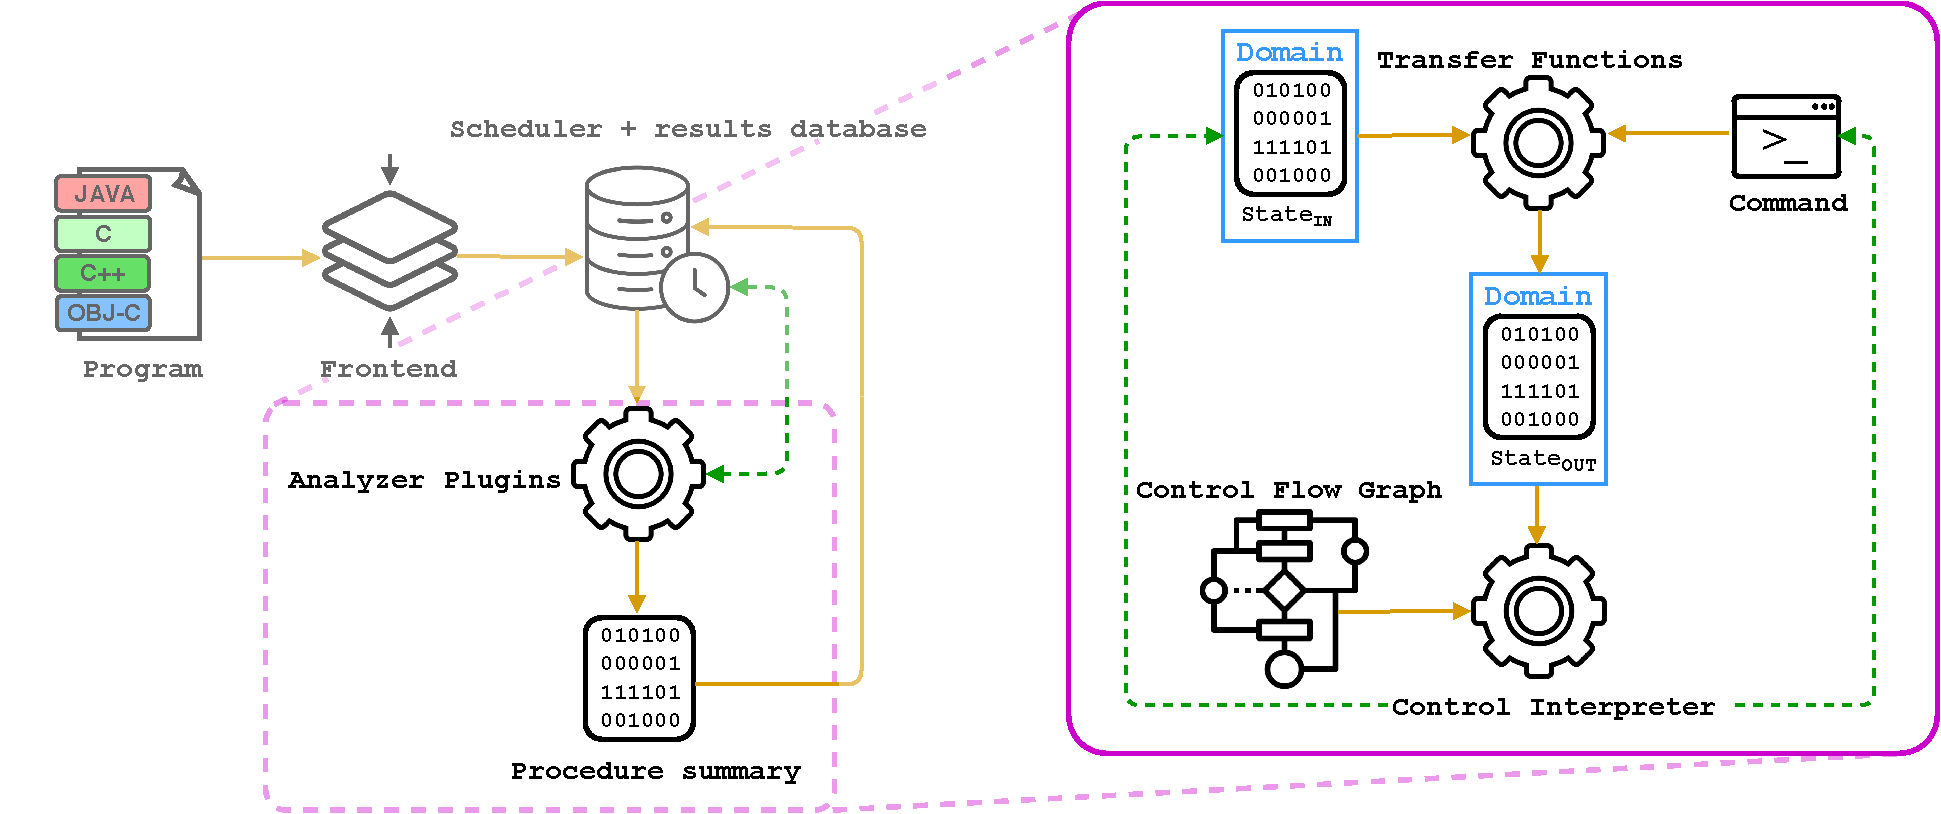
\includegraphics[scale=1.0]{img/infer.pdf}
\end{minipage}
\hspace{1em}
\begin{minipage}[T]{.35 \linewidth}
    \begin{center}
        
\includegraphics[scale=.7]{img/infer-logo.png}
    \end{center}

    \begin{itemize}
        \normalsize

        \item
            \textbf{Open-source} static analysis framework.

        \item
            Suite of \textbf{modular} static analysers.
            \begin{itemize}
                \small

                \item
                    Checks for, e.g., buffer overflow, thread-safety,
                    null-dereferencing or memory leaks.
            \end{itemize}

        \item
            Follows principles of \textbf{compositionality.}
            \begin{itemize}
                \small

                \item
                    \textbf{Highly scalable.}

                \item
                    Analysis of \textbf{code changes} only.
            \end{itemize}
    \end{itemize}
\end{minipage}
\vspace{-.5em}
}


%--------------------------------------------------------
%--------------------------------------------------------
%--------------------------------------------------------
%--------------------------------------------------------
\block{\textsc{Looper}: Worst-Case Cost Analyser}{
\begin{minipage}{0.33 \linewidth}
    \vspace{-9.5em}

    \begin{itemize}
        \normalsize

        \item
            Recast of the \textbf{Loopus} tool in Infer.
            \vspace{0.3cm}

        \item
            Supports \textbf{amortized complexity} analysis.
            \vspace{0.3cm}
        \item
            Based on recursive \textbf{transition} and
            \textbf{variable} bounds computation.
            \vspace{0.3cm}

        \item
            Current prototype is \textbf{intra-procedural} only.
            \vspace{0.3cm}

        \item
            Promising results on selected examples
            in comparison to \textbf{Cost} Infer checker.
    \end{itemize}
\end{minipage}
\hspace{0.5em}
\begin{minipage}{.19 \linewidth}
    \vspace{-9.5em}
    \centering\normalsize\textbf{Experimental evaluation} \\[0.5em]
    \small

    \def\arraystretch{1.1}
    \begin{tabular}{crR{2.7cm}R{2cm}}
        & Bound & \textbf{Looper} & \textbf{Cost} \\
        \hline

        \#1 & $n$ & \bad{$\bm{2n}$} & \bad{$\bm{n^2}$} \\
        \hline

        \#2 & $2n$ & \good{$\bm{2n}$} & \bad{$\bm{5n}$} \\
        \hline

        \#3 & $4n$ & \bad{$\bm{5n}$} & \bad{$\bm{\infty}$} \\
        \hline

        \#4 & *$n^2$ & *\good{$\bm{n^2}$} & \bad{$\bm{\infty}$} \\
        \hline

        \#5 & $2n$ & \good{$\bm{2n}$} & \bad{$\bm{12n}$} \\
        \hline

        \#6 & *$n$ & *\good{$\bm{n}$} & \bad{$\bm{\infty}$} \\
        \hline

        \#7 & $2n$ & \good{$\bm{2n}$} & \bad{$\bm{\infty}$} \\
        \hline

        \#8 & $2n$ & \good{$\bm{2n}$} & \bad{$\bm{\infty}$} \\
        \hline
    \end{tabular}
\end{minipage}
\begin{minipage}{.29 \linewidth}
    \vspace{-9.5em}
    \centering\normalsize\textbf{Bound computation} \\[1.3em]
    \def\arraystretch{1.3}
    \small

    \begin{tabular}{rl}
        \hline

        \multirow{2}{*}{
        \red{$T\mathcal{B}(\bm{\tau_2})$}} &
        $\rightarrow \blue{\mathtt{Incr}(\bm{j})} +
        T\mathcal{B}(\tau_0) \times
        \max(V\mathcal{B}(0) + 0, 0)$ \\
        &$\rightarrow \green{\bm{n}} + 1 \times 0 =
        \green{\bm{n}}$\Bstrut \\
        \hline

        $\blue{\mathtt{Incr}(\bm{j})}$ &
        $\rightarrow$ \purple{$T\mathcal{B}(\bm{\tau_1})$} $\times 1
        = \green{\bm{n}} \times 1 = \green{\bm{n}}$ \Tstrut\Bstrut \\
        \hline

        \multirow{2}{*}{\purple{$T\mathcal{B}(\bm{\tau_1})$}} &
        $\rightarrow \mathtt{Incr}(i) +
        T\mathcal{B}(\tau_0) \times
        \max(\green{V\mathcal{B}(\bm{n})} + 0, 0)$ \Tstrut \\
        & $\rightarrow 0 + 1 \times \max(\green{\bm{n}} + 0, 0) =
        \green{\bm{n}}$ \Bstrut \\
        \hline

        $\green{V\mathcal{B}(\bm{n})}$ &
        $\rightarrow \green{\bm{n}}\quad\text{(formal
        parameter)}$\Tstrut\Bstrut \\
        \hline
    \end{tabular}
\end{minipage}
\hspace{0.2em}
\begin{minipage}[t]{.15 \linewidth}
    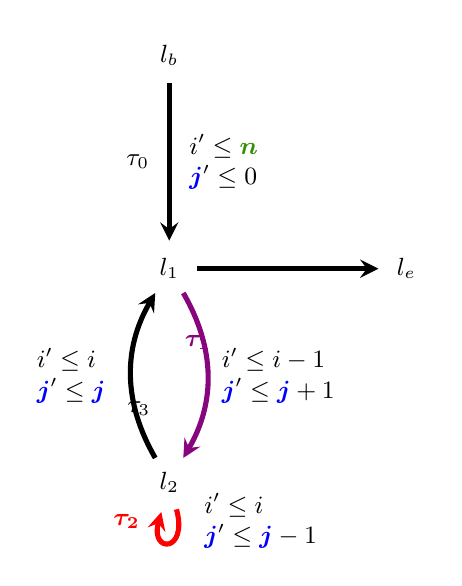
\begin{tikzpicture}[
        > = stealth, % arrow head style
        shorten > = 0pt,
        auto,
        node distance = 2cm, % distance between nodes
        line width=0.65mm, % line style
        font=\small\bfseries
    ]
        \tikzstyle{every state}=[
            draw = white,
            thick,
            fill = white,
            minimum size = 4mm,
        ]
        \node[state] (lb) {$l_b$};
        \node[state] (l1) [below=2cm of lb] {$l_1$};
        \node[state] (l2) [below=2cm of l1] {$l_2$};
        \node[state] (le) [right=2.3cm of l1] {$l_e$};

        \path[->] (lb) edge
        node[left=3pt, pos=0.5]{$\tau_0$}
        node[align=left, right=3pt, pos=0.5] {
        $i' \leq \green{\bm{n}}$\\
        $\blue{\bm{j}}' \leq 0$} (l1);

        \path[->] (l1) edge[draw=purple, bend left]
        node[left=-7pt, pos=0.3]{\purple{$\bm{\tau_1}$}}
        node[align=left, right=1pt] {
        $i' \leq i - 1$\\
        $\blue{\bm{j}}' \leq \blue{\bm{j}} + 1$} (l2);

        \path[->] (l2) edge[bend left]
        node[pos=0.3, right=-7pt]{$\tau_3$}
        node[align=left, left=5pt] {
        $i' \leq i$\\
        $\blue{\bm{j}}' \leq \blue{\bm{j}}$} (l1);

        \path[->] (l1) edge node {} (le);

        \path[->] (l2) edge[draw=red,loop below]
        node[align=left, right=5pt, pos=0.1] {
        $i' \leq i$\\
        $\blue{\bm{j}}' \leq \blue{\bm{j}} - 1$}
        node[left=3pt, pos=0.9] {\red{$\bm{\tau_2}$}} (l2);
    \end{tikzpicture}
\end{minipage}
}


%--------------------------------------------------------
%--------------------------------------------------------
%--------------------------------------------------------
%--------------------------------------------------------
\block{\textsc{Atomer}: Atomicity Violations Analyser}{
\normalsize
\begin{minipage}{.55 \linewidth}
    \centering
    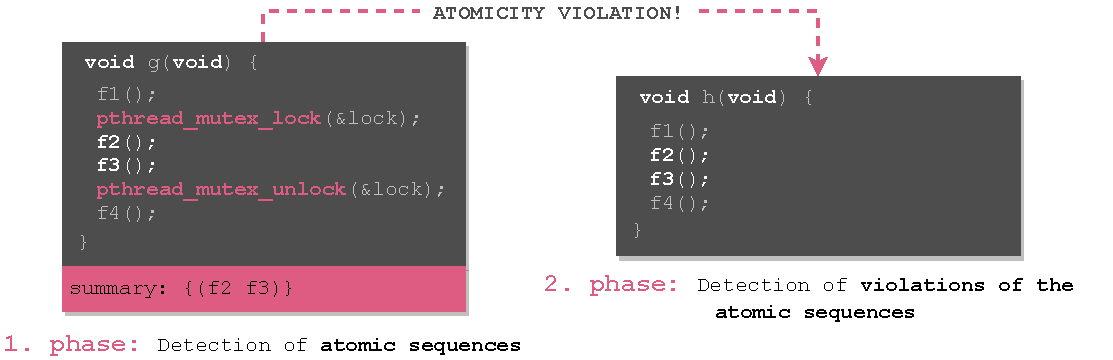
\includegraphics[width=1\linewidth]{img/atomer.pdf}
\end{minipage}
\begin{minipage}{0.41 \linewidth}
    \begin{itemize}
        \item
            Finds atomicity violations for \textbf{sequences
            of functions}.
            \vspace{0.4cm}

        \item
            Based on assumption that sequences executed \textbf{once
            atomically} should be executed \textbf{always atomically}.
            \vspace{0.4cm}

        \item
            Adapts the technique of \textbf{contracts for concurrency}.
            \vspace{0.4cm}

        \item
            Targets \textbf{C/C++} programs that uses
            \textbf{Pthreads} locks.
    \end{itemize}
\end{minipage}
}


%--------------------------------------------------------
%--------------------------------------------------------
%--------------------------------------------------------
%--------------------------------------------------------
\block{\textsc{L2D2}: Low-Level Deadlock Detector}{
\begin{minipage}{0.28 \linewidth}
    \vspace{-10em}

    \begin{itemize}
        \normalsize

        % \item
            % Based on \textbf{Lockset} analysis.

        \item
            \textbf{11.4\,MLOC} derived from
            
\includegraphics[scale=.2]{img/debian-logo-small.jpeg}.%
            \vspace{0.5cm}

        \item
            \textbf{100\,\% deadlock detection} rate.
            \vspace{0.5cm}

        \item
            Roughly \textbf{11\,\% FP} rate.
            \vspace{0.5cm}

        % \item
            % Experiments took only \textbf{2 hours}.

        \item
            Less than \textbf{1\,\%} of the time of \texttt{CPROVER}.
    \end{itemize}
\end{minipage}
\hspace{.5em}
\begin{minipage}{0.25 \linewidth}
    \vspace{-10em}
    \textbf{Experimental evaluation} \\

    \normalsize
    \begin{tabular}{lrr}
        & L2D2 & CPROVER \\
        \hline

        Deadlocks & \good{8} & \good{8 }\\
        False Positives & \bad{104} & \bad{114} \\
        No deadlocks & \good{810} & \good{292} \\
        Failed Cases & \bad{80} & \bad{588} \\
        \hline

        \textbf{Total} & \textbf{1002} & \textbf{1002}
    \end{tabular}
\end{minipage}
\begin{minipage}[t]{.4 \linewidth}
    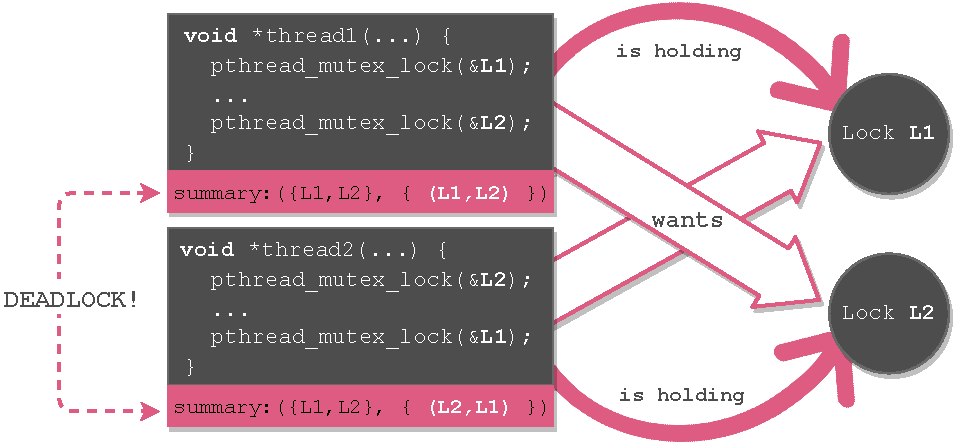
\includegraphics[width=23em, height=10em]{img/l2d2.pdf}
\end{minipage}
}


%--------------------------------------------------------
%--------------------------------------------------------
%--------------------------------------------------------
%--------------------------------------------------------
\node[
    above right,
    outer sep=0pt,
    minimum width=\paperwidth,
    draw,
    align=center,
    fill=footercolor,
    font=\normalsize,
    minimum height=70pt
] at (bottomleft) {
    \textcolor{white}{
        The work is supported by the H2020 ECSEL project
        \textbf{\large{AQUAS}}: Aggregated Quality Assurance
        for Systems and \textbf{\large{VeriFIT}} group (BUT FIT).
    }
};


\end{document}
